%!TEX root = ../dokumentation.tex

\chapter{Implementierung}

\section{Ausgangslage}

\section{Simulation als Datenproduktion}
Strecke modelieren
Man kann in der Simulation Strecken aufbauen. Dazu wird auch zu jeder Strecke eine Ideallinie für das Fahrzeug generiert.
Diese Strecke besteht aus einer Liste von Punkten.
Das Modul AutomaticDrive kann genutzt werden damit das Fahrzeug entlang dieser Strecke fährt.
Das Fahrzeug fährt dann aber in gerader Linie von Punkt zu Punkt. 
Dadurch kommt es in Kurven zu einem ruckeligen Fahrverhalten.
WIE LÖST MAN DAS PROBLEM. INTERPOLATION IN KURVEN BEI AUTODRIVE

Die Positionierung und Orientierung funktioniert mit dem Hinterachsenmittelpunkt H als Basis.
Das Fahrzeug fährt indem der Punkt H mit einer konstanten Geschwindigkeit entlang der Fahrspur fährt.
Die Orientierung des Fahrzeugs ist so definiert, dass das Fahrzeug am Punkt H eine Tangente zur Fahrspur bildet.
Die Tangente kann mit einer Funktioner der Datenstruktur der Fahrspur erechnet werden. 
In einer Kurve kann das Fahrzeug dann so aussehen:

\begin{wrapfigure}{r}{.4\textwidth}
    \centering
    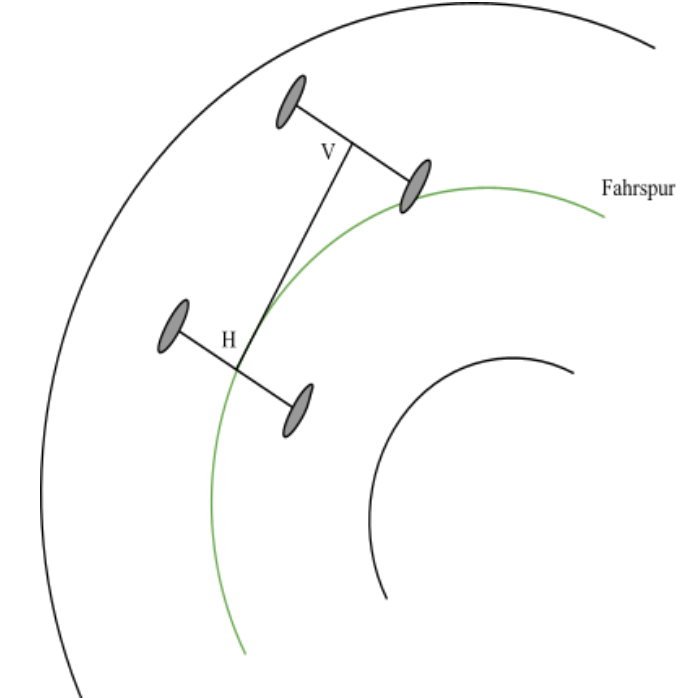
\includegraphics[height=.35\textwidth]{AutoDrive.png}
    \vspace{-15pt}
    \caption{BlaBla\footnotemark}
\end{wrapfigure}

Positionierung und Rotation um Punkt H hat sich als realitätsnah erwiesen, da die Kamera, die vorne am Fahrzeug montiert ist, in den Kurven ein ähnliches Bild geliefert hat wie das echte Fahrzeug.


Kamera entlang der Strecke fahren lassen

Um Algorithmen und Model in der Spurerkennung und Situationsklassifizierung zu verifizieren und verbessern, 
benötigt der Auto drive noch eine Möglichkeit den Lenkwinkel auszugeben.
Für den AutomaticDrive nehmen wir ein paralleles Lenksystem an.
Punkt V nach H. $\vec{VH}$ 

Die Vorderräder sind ausgerichtet entlang der Tangente VT am Punkt V zur Fahrspur.
Der Lenkwinkel $\beta$ ist der Winkel zwischen $\vec{VH}$ und $\vec{Lenkrichtung}$. 

\begin{wrapfigure}{r}{.4\textwidth}
    \centering
    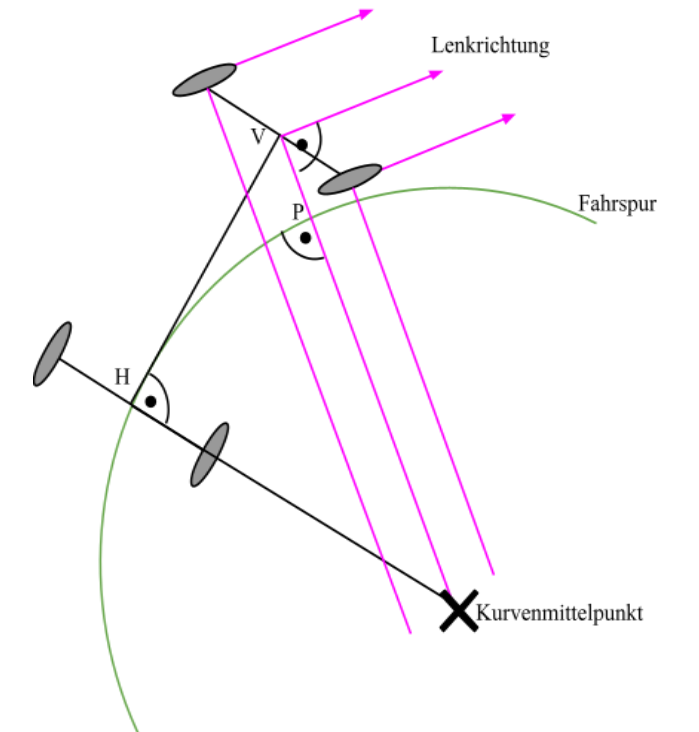
\includegraphics[height=.35\textwidth]{ParallelSteering.png}
    \vspace{-15pt}
    \caption{BlaBla\footnotemark}
\end{wrapfigure}

\section{Kamera}
Auflösung, Position, FoV eingestellt.

Die Auflösung der Kamera ist 2x2 Pixel.
Die Position und Orientierung der Kamera wird genau ermittelt, um die simulierte Kamera an die selbe Position zu bringen.
 

Problem: Für die IPM umrechnung muss der Kamerafeed sehr genau den echten wiederspiegeln.
Neue matrix wäre eine Scheiß Lösung.


\section{statische Fortbewegung}
Problem: Lenkwinkel muss irgendwie in eine Transformation des Fahrzeugs umgewandelt werden.
Der genaue Lösung wäre eine dynamische Simulation der Räder und Lenkung.
Dies war nicht so einfach abzustimmen, da sich die Simulation anders Verhalten hat als das echte Fahrzeug.
Vorläufige Lösung: Eine Rechnung die die Transformation abschätzt, aber sehr genau ist bei kleinen Lenkwinkel und hoher Fps.

Gegeben ist der Lenkwinkel alpha
Die Geschwindigkeit des Fahrzeugs v
Der daraus resultierende Vektor Lenkrichtung steering
Position des Fahrzeugs p
Orientierung des Fahrzeugs und der daraus resultierende Vektor direction

Als erstes wird aus dem Lenkwinkel alpha der Vektor steering bestimmt.
Danach wird die neue Position pNeu bestimmt mit pNeu = p + steering * (deltaTime * v)
Die neue Orientierung des Fahrzeugs directionNeu wird erechnet mit directionNeu = direction rotieren um k*alpha
dabei ist k Abhängig von der gefahrenen Strecke, sowie der Fahrzeuglänge.

\section{dynamische Fortbewegung}
Vier drehende Räder, Antrieb, Lenkung vorne.
Problem mit, Kräften, massen, Kollision...
on...

Die Räder des Fahrzeugs werden definiert innerhalb einem Link.
Jeder der vier Links besitzt eine visuelle Komponente und ein Kollisions-Komponente.
Das visuelle Objekt und das Kollisions-Objekt stimmen überein, beide definieren den gleichen Zylinder.
Jeder physikalisch simulierte Link benötigt einen inertial-Tag.
Dieser definiert die Masse "mass" und die Massenverteilung als inertia Tensor "inertia".

Damit sich ein Rad drehen kann, wird es mit einem Joint an dem Fahrzeug befestigt.
Der Joint definiert die beiden Links die verbunden werden sollen: child und parent.
Der Typ des Joints ist für die Räder "continuos". Das bedeuted, dass sich die Räder ohne Einschränkung um eine Achse drehen können.
Der Joint definiert außerdem die Position und Orientierung der Achse.

DiskJoints.

Um die Räder und die Länkung zu steuern, benötigt es einen Motor. 
Für urdf gibt es hierfür Actuator und Transmissions.
Eine Transmission verbindet einen Actuator mit einem Joint. 
ACTUATOR TRANSMISSIONS CODE HIER

Controller
Um die Actuator zu steuern kann man das Package ros\_control nutzten.
Dies bietet eine Reihe verschiedener Controller.
Controller können einen Actuator nach PID-Steuerung steuern.
Um die Controller zu benutzen wird ein neues Package erstellt.
Das Package $/simulation/src/gazebo_controller$ beinhaltet eine Launchdatei und eine Parameterdatei.
Die Parameterdatei definiert die vier verschiedenen Controller.
Zwei für den Hinterradantrieb und zwei für die Vorderlenkung.
Die Controller für den Antrieb sind JointVelocityController, die Controller für die Lenkung sind JointPositionController.
Von dem Antrieb soll die Geschwindigkeit gesteuert werden, von der Lenkung soll die Position bzw. die Rotation gesteuert werden.
In der Parameterdatei werden auch die zugehörigen Joints und die PID Parameter definiert.
Die Launchdatei nutzt die Parameterdatei und lädt damit die Controller über einen controller\_spawner.
Die Launchdatei wird in der master.launch-Datei wie folgt aufgerufen:
\begin{lstlisting}
<include if="\$(eval include_automatic_drive == false)" file="\$(find gazebo_controller)/launch/robot_control.launch"></include>
\end{lstlisting}
Die Controller werden nur initialisiert, wenn AutomaticDrive nicht genutzt wird.

\subsection{PID Regelung}
PID Regler werden eingesetzt um eine bestimmte Regelgröße zu regeln. 
Der Regler vergleicht den Soll- und Istwert der Regelgröße und versucht deren Differenz zu minimieren.
Dieses Ziel verfolgt er über drei Komponenten: 
Die Proportional-Komponente, welche abhängig von der aktuellen Differenz zwischen Ist- und Sollwert ist.
Die Integral-Komponente, welche abhängig von der vergangenen Differenz zwischen Ist- und Sollwert ist.
Die Differentail-Komponente, welche abhängig von der zukünftigen Differenz zwischen Ist- und Sollwert ist.
Wie groß der Einfluss der jeweiligen Komponente ist lässt sich über die Parameter P,I und D steuern.
\cite{PIDRegler:2020}

BILD PID IST SOLL IN SIMU

\subsection{Ackerman Lenkung}
Ziel der Simulation ist es bei gegebenem Lenkwinkel und Geschwindigkeit das Fahrzeug entsprechend zu bewegen.
Die Geschwindigkeit wird an die zwei Geschwindigkeitscontroller gegeben.
Der Lenkwinkel wird an die zwei Lenkcontroller gegeben.
Hierbei treten jedoch zwei Probleme auf:

Wenn sich beide Hinterräder in der genau gleichen Geschwindigkeit drehen, kann es zu Problemen in Kurven kommen.
Das äußere Rad muss eine längere Strecke in der gleichen Zeit wie das innere Rad fahren. 
Dadurch kann es zu ungewünschten Kräften und Rutschen kommen.
Im echten Fahrzeug wird dieses Problem durch ein Differentialgetriebe gelöst.
In der Simulation hat sich das als kein großes Problem erwiesen und es bleibt erstmal bei zwei Controllern mit der genau gleichen Geschwindigkeit, auch in den Kurven.

Das zweite Problem ist die Lenkung. 
Wenn man den Lenkwinkel direkt an beide Controller weitergibt hat man eine Parallellenkung.
Das Fahrzeug mit Parallellenkung sieht in einer Kurve so aus:  
\begin{wrapfigure}{r}{.4\textwidth}
    \centering
    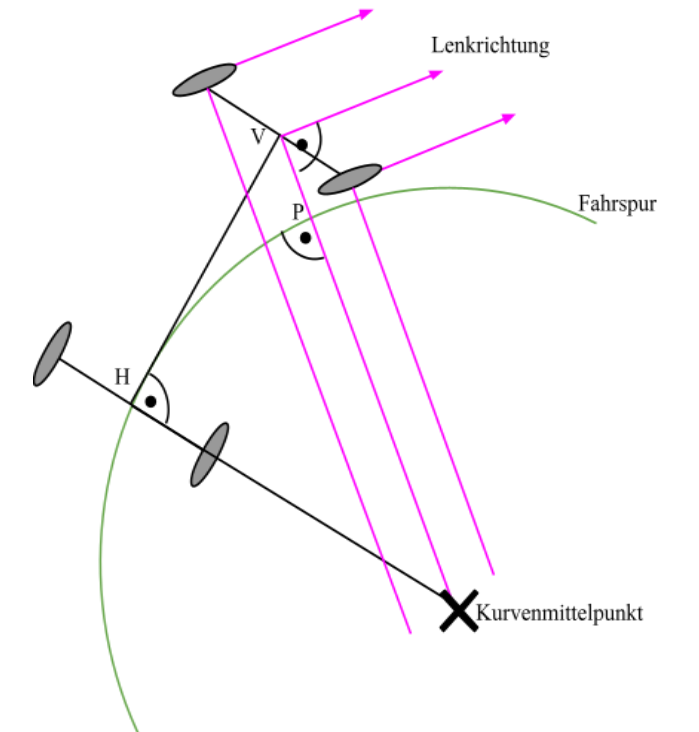
\includegraphics[height=.35\textwidth]{ParallelSteering.png}
    \vspace{-15pt}
    \caption{BlaBla\footnotemark}
\end{wrapfigure}
Das Fahrzeug fährt um den Kurvenmittelpunkt herum. 
Wenn ein Rad eine Kurve fährt, ist es so ausgerichtet, dass es entlang einer Tangenten auf dem Kreis um den Kurvenmittelpunkt fährt.
Die Hinterräder des Fahrzeugs fahren um den Kurvenmittelpunkt.
Die Vorderräder sind allerdings nicht entlang eines Kreises um den Kurvenmittelpunkt orientiert sondern parallel zur Lenkrichtung.
Die Lenkrichtung geht aus vom Vorderachsenmittelpunkt V.
Dies kann ebenfalls zu Rutschen und ungewollten Kräften auf Räder und Lenkung führen.
Um das zu verhindern wird im echten Fahrzeug eine Ackermann-Lenkung verwendet. 
Diese sieht in einer Kurve so aus:
\begin{wrapfigure}{r}{.4\textwidth}
    \centering
    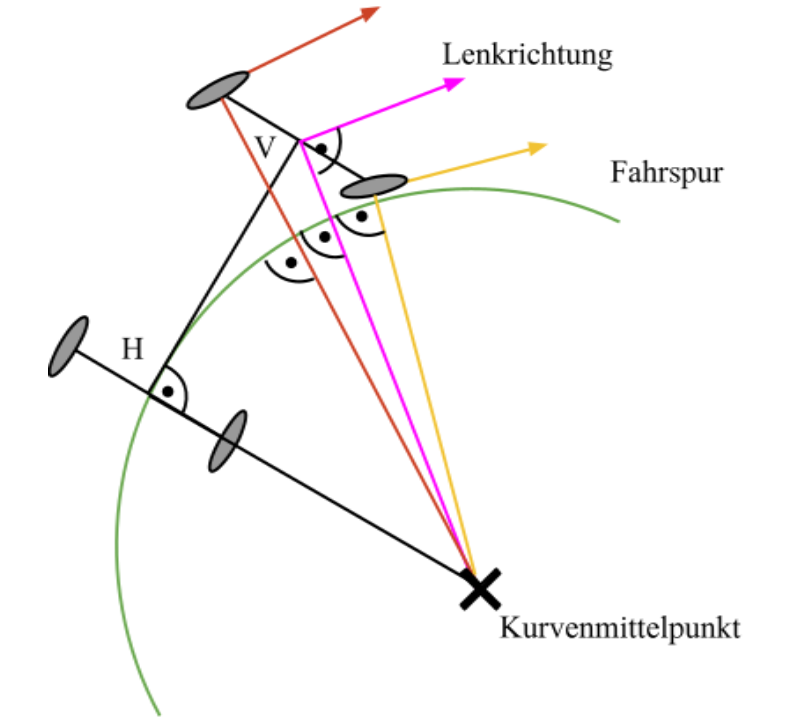
\includegraphics[height=.35\textwidth]{Ackermann.png}
    \vspace{-15pt}
    \caption{BlaBla\footnotemark}
\end{wrapfigure}
Im Gegensatz zu Parallellenkung sind nun auch die Vorderräder entlang einem Kreis um den Kurvenmittelpunkt ausgerichtet.
Das linke Rad hat nun einen anderen Winkel wie das rechte Rad.

Wie die Ackerman-Lenkung, per Hardware, im echten Fahrzeug umgesetzt ist hier unwichtig.
Um die Ackerman-Lenkung zu simulieren, können aus einem gegebenen Lenkwinkel, jeweils der Winkel für das rechte und linke Rad berechnet werden.

\begin{wrapfigure}{r}{.4\textwidth}
    \centering
    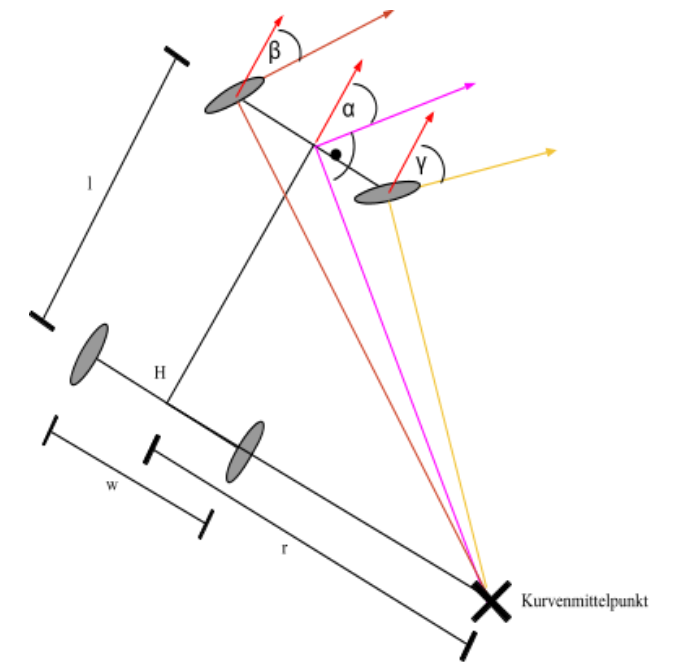
\includegraphics[height=.5\textwidth]{AckermannBerechnung.png}
    \vspace{-15pt}
    \caption{BlaBla}
\end{wrapfigure}

Ziel ist es die Winkel $\beta$ und $\gamma$ zu bestimmen.
Gegeben ist der Lenkwinkel am Vorderachsenmittelpunkt $\alpha$. 
Mit der Fahrtrichtung und $\alpha$ lässt sich die pinke Linie konstruieren. 
Außerdem ist gegeben dass die Hinterachse auf einer Geraden mit dem Kurvenmittelpunkt liegt.
Der Schnittpunkt der pinken Linie und dieser Geraden ist der Kurvenmittelpunkt.
Die Strecke von H zum Kurvenmittelpunkt wird definiert als r.
Die Strecke w ist der Radabstand zwischen den rechten und linken Rädern.
Die Strecke l ist der Radabstand zwischen den vorderen und hinteren Rädern.
Aus der Pinken Strecke und den Strecken r und l bildet sich ein Dreieck mit rechtem Winkel bei H.
Daraus folgt 
\begin{equation} \label{eq:1}
    \tan(\alpha) = \frac{l}{r}
\end{equation}
Wenn man den Punkt H um $\frac{w}{2}$ nach rechts und links verschiebt kann man zwei weitere rechtwinklige Dreiecke konstruieren.
Diese beinhalten jeweils die braune oder gelbe Strecke. 
Aus den zwei Dreiecken gehen folgende Gleichungen hervor:
\begin{equation} \label{eq:2}
    \tan(\beta) = \frac{l}{r-w/2} 
\end{equation}
\begin{equation}  \label{eq:3}
    \tan(\gamma) = \frac{l}{r+w/2} 
\end{equation}
Umformung Gleichung \ref{eq:1}
\begin{equation} \label{eq:4}
    r = \frac{l}{\tan(\alpha)}
\end{equation}
Setzte man Gleichung \ref{eq:4} in Gleichung \ref{eq:2} ein so erhält man
\[ \tan(\beta) = \frac{l}{\frac{l}{\tan(\alpha)}-w/2}\] 
\[ \iff \beta = \arctan(\frac{l}{\frac{l}{\tan(\alpha)}-w/2})\] 
Analog dazu erhält man die Gleichung für $\gamma$
\[ \gamma = \arctan(\frac{l}{\frac{l}{\tan(\alpha)}+w/2})\] 
Mit diesen zwei Gleichungen lassen sich die Winkel $\beta$ und $\gamma$ bestimmen.
Die Radabstände l und w sind fest in der Simulation definiert.
Beide individuelle Lenkwinkel $\beta$ und $\gamma$ sind nur von einer Variablen abhängig: Dem Lenkwinkel am Vorderachsenmittelpunkt $\alpha$.
\cite{ackerman:2021}